\def\year{2015}
\def\thetitle{Wide Retrofitting: Breadth of Knowledge Improves Word Vectors}

% Update this when our score changes.
\def\scoreRW{.584}
\def\scoreMEN{.860}

\documentclass[11pt]{article}
\usepackage{acl2012}
\usepackage{times}
\usepackage{latexsym}
\usepackage{amsmath}
\usepackage{multirow}
\usepackage{pgfplots}
\pgfplotsset{compat=1.9}
\usepackage{booktabs}
\usepackage{CJKutf8}
\usepackage{url}
\setlength{\pdfpagewidth}{8.5in}
\setlength{\pdfpageheight}{11in}
\pdfinfo{
/Title \thetitle
/Author Rob Speer, Joshua Chin, and Catherine Havasi}
%\setcounter{secnumdepth}{0}
\bibliographystyle{acl2012}

\title{\thetitle}
%\author{Robert Speer\\
%    Luminoso Technologies, Inc.\\
%    675 Massachusetts Ave.\\
%    Cambridge, MA 02139\\
%    \texttt{rspeer@luminoso.com}
%\And
%    Joshua Chin\\
%    {\em academic address goes here}
%\And
%    Catherine Havasi\\
%    Luminoso Technologies, Inc.\\
%    675 Massachusetts Ave.\\
%    Cambridge, MA 02139\\
%    \texttt{havasi@luminoso.com}
%}

\begin{document}
\maketitle
\begin{abstract}

A currently successful approach to computationally represent the meanings of
words is to represent them as vectors (embeddings) in a machine-learned vector
space. These embeddings are often evaluated on their ability to identify
similar or related words like a human would. In this paper, we show the
effectiveness of combining existing embeddings learned by GloVe
\cite{pennington2014glove} with structured knowledge from the semantic network
ConceptNet 5 \cite{speer2012conceptnet}, merging their information into a common
representation using an extension of the ``retrofitting'' technique
\cite{faruqui2015retrofitting}. The resulting vector space has a larger vocabulary
than either source, can represent word meanings in multiple languages, and
achieves state-of-the-art performance on word similarity evaluations.
Its score of $\rho = \scoreRW{}$ on an evaluation of rare words
\cite{luong2013rw} is 13.6\% higher than the previous best known system.

\end{abstract}

\section{Introduction}

Vector space models are an effective way to express the meanings of
natural-language terms in a computational system. These models are created
using machine-learning algorithms that attempt to represent words or phrases as
vectors in a high dimensional space, such that the cosine similarity of any two
words corresponds to their semantic similarity. This kind of vector space has
been used in applications such as search and topic detection, dating back to
the introduction of latent semantic analysis \cite{deerwester1990indexing}.  In
recent years, there has been a surge of interest in natural-language
embeddings, as machine-learning techniques such as
\newcite{mikolov2013word2vec}'s word2vec and \newcite{pennington2014glove}'s
GloVe have begun to show dramatic improvements.

A recent paper from \newcite{faruqui2015retrofitting} introduced a technique
known as ``retrofitting'', which combines embeddings learned from the
distributional semantics of unstructured text with a source of structured
connections between words. The combined embedding achieves performance on
word-similarity evaluations superior to either source individually.

While the original formulation of retrofitting operates on the intersection of
the vocabularies, we modify it to operate on the union. This allows retrofitting
to expand the vocabulary of the embedding instead of shrinking it, and allows it
to benefit from semantic links that must be followed for multiple steps to reach
a term in the original vocabulary. We refer to this modified procedure as
``wide retrofitting''.

By combining our modified version of retrofitting with some subtle but important
normalizations to the input data, we achieve state-of-the-art performance using
the distributional embeddings learned by GloVe \cite{pennington2014glove} from
the Common Crawl\footnote{\url{https://commoncrawl.org/}} with the structured word and phrase
associations in ConceptNet \cite{speer2012conceptnet}. These new embeddings
outperform many other recently-published methods on word-similarity
evaluations\footnote{Some methods distinguish word similarity from word
{\em relatedness}. ``Coffee'' and ``mug'', for example, are quite related,
but not actually similar because coffee is not {\em like} a mug. In this paper,
however, we conflate similarity and relatedness into the same metric, as most
evaluations do.} over both common and rare words.

In all, we take a three-pronged approach to improving word similarity
judgments. We will show that each of these methods improves performance on
word-similarity evaluations, and that the best results comes from applying all
of them at once:

\begin{itemize}
\item Normalizing the features of the GloVe matrix with $L_1$ instead of $L_2$
    normalization, increasing the weight of more selective features
\item Transforming the matrix labels with a text ``standardization'' function,
    unifying variations and inflections of the same word
\item Applying wide retrofitting to introduce a broad variety of
    structured semantic knowledge from ConceptNet 5.4
\end{itemize}

The results provide state-of-the-art performance on word similarity tasks. We
consider this to show the usefulness of expanding a vector space representation
by giving it multiple ways to learn a word. ``Wide retrofitting'' could be
considered an ensemble method for learning a vector space representation
instead of a classifier.

\section{Background}

\subsection{GloVe}

GloVe \cite{pennington2014glove} is an unsupervised learning algorithm that
learns vector representations of words, such that the dot product of two words'
vectors is approximately equal to the logarithm of their co-occurrence count.
The algorithm operates on a global word-word co-occurrence matrix, and
solves an optimization problem to learn a vector for each word, a separate
vector for each context (although the contexts are also words), and a bias
value for each word and each context. Only the word vectors are used for
computing similarity.

Learning processes such as GloVe produce results that can conveniently be
re-used in other projects, simply by re-using the matrix of word embeddings.
The embeddings that GloVe learns from data sources such as the Common Crawl are
distributed on the GloVe web
page\footnote{\url{http://nlp.stanford.edu/projects/glove/}}.

\subsection{ConceptNet}
ConceptNet \cite{speer2012conceptnet} is a semantic network of terms
connected by labeled relations. Its terms are words or multiple-word phrases
in a variety of natural language. For continuity with previous work,
these terms are often referred to as {\em concepts}.

ConceptNet originated as a machine-parsed version of the early crowd-sourcing
project called Open Mind Common Sense (OMCS) \cite{singh2002omcs}, and has expanded
to include several other data sources, both crowd-sourced and expert-created,
by unifying their vocabularies of terms into a single representation.
The data sources included in ConceptNet 5.4 are:

\begin{itemize}
\item Knowledge collected as English sentences on the original OMCS website,
    and later parsed with a pattern-matching parser
\item OMCS projects that collected similar sentences in Portuguese
    \cite{anacleto2006portuguese},
    Dutch \cite{eckhardt2008kid}, and some Korean and Japanese
    \cite{chung2006globalmind}
\item ``Games with a purpose'' that have collected relational knowledge, such as
    Verbosity \cite{vonahn2006verbosity} in English, {\em nadya.jp}
    \cite{nakahara2011nadya} in Japanese, and the PTT pet game \cite{kuo2009petgame}
    in Taiwanese Chinese
\item WordNet 3.0 \cite{miller1998wordnet}
\item A parsed version of Wiktionary's entries whose target language is English or
      German \cite{wiktionary2014en} \cite{wiktionary2014de}, generated
      by a parser developed as part of the ConceptNet 5.4 codebase
\item JMDict \cite{breen2004jmdict}, a Japanese multilingual dictionary
\item OpenCyc \cite{matuszek2006cyc} as represented in Umbel \cite{bergman2008umbel}
\end{itemize}

ConceptNet also includes a mapping of DBPedia \cite{auer2007dbpedia} into
its vocabulary, but it is not used for word associations, so its presence does
not affect the results in this paper.

\section{Methods}

\newcite{faruqui2015retrofitting} introduced the ``retrofitting'' procedure,
which adjusts dense matrices of embeddings (such as the GloVe output) to take
into account external knowledge from a sparse semantic network. They used PPDB
\cite{ganitkevitch2013ppdb} as an external source of semantic knowledge. We
found using ConceptNet as the external knowledge source to be more effective,
and that further marginal improvements could be achieved on some evaluations by
combining ConceptNet and PPDB.

We create a matrix that assigns embeddings in a 300-dimensional vector
space to terms by combining data from ConceptNet and GloVe. The resulting word
embeddings incorporate the strengths of both ConceptNet and GloVe, and extend
their vocabulary to the union of ConceptNet and GloVe, allowing embeddings that
were originally only trained on English to be extended to other languages.

\subsection{Standardizing Text}

As \newcite{levy2015embeddings} note,
``[\ldots] much of the performance gains of word embeddings are due to certain
system design choices and hyperparameter optimizations, rather than the
embedding algorithms themselves.'' While it is presented as a negative result,
this simply emphasizes the importance of these system design choices.

Indeed, we have found that choices about how to handle text have a significant
impact on evaluation results. Additionally, we can only properly combine two
resources with a method such as retrofitting if their string representations
are comparable to each other.

The operations we apply to text would usually be called ``normalization'',
but that word also refers to the scaling operations we will be applying to
vectors, so both here and in the code we call it ``standardization'' instead.

ConceptNet 5.4 uses a particular sequence of operations to standardize its
text, and we have reproduced these operations in the code that supports this
paper.  The operations include tokenizing the text using a Unicode-aware
regular expression, reducing English words to their root forms using a
modification of WordNet's Morphy algorithm, removing a very small list of
stopwords (``a'', ``an'', and ``the''), replacing spaces and slashes with
underscores, lowercasing the text, and tagging the result with its language.

As an example, in ConceptNet, the text ``give an example'' becomes the standardized form
{\tt /c/en/give\_example}.

The 42-billion-token version of GloVe, whose results are published in
\cite{pennington2014glove}, applies some more minimal standardizations that do
not include stemming. The 840-billion-token version applies almost no
standardization, and in particular it does not lowercase its words.

\subsubsection{Aligning ConceptNet and GloVe}

Because ConceptNet's standardization process is stronger than GloVe's, we align them
by applying the ConceptNet standardizations to the GloVe labels as well, turning
its tokens into ConceptNet URIs. The GloVe tokens are assumed to be in English.

This has the effect that many separate rows of the GloVe matrix get the same
label, such as when the same word appears with a different capitalization.
We considered a few options for dealing with these merged labels:

\begin{enumerate}
\item Keep only the row with the highest frequency in GloVe.
\item Average the rows together.
\item Take a weighted average that favors higher-frequency rows.
\end{enumerate}

% NOTE: Avril wants us to describe how many rows change due to standardization

The weighted average turns out to be the best approach, as our evaluation will
show. The multiple rows contain valuable data that should not simply be
discarded, but lower-frequency rows tend to have lower-quality data.

The word frequency data is not distributed with the GloVe matrix, but
the rows are clearly in descending order of frequency. We approximate the
frequency distribution by assuming that the tokens are distributed according to
Zipf's law \cite{zipf1949human}: the $n$th token in rank order has a frequency
proportional to $1/n$.

In order to evaluate the combined word vectors, it is necessary for us to apply
the same standardizations to the evaluation data. A drawback to this
standardization process is that we will not be able to evaluate the result on
\newcite{mikolov2013word2vec}'s syntactic analogy task, as many of
the analogies would become trivial analogies of the form
``A is to A as B is to B''.

Due to a quirk in some of the evaluation data, we must apply one more
standardization to all labels, even though it is not necessary in ConceptNet or
in GloVe. The Spanish translations of word-similarity evaluations
\cite{hassan2009crosslingual} are written without any accents on the
letters, such as ``telefono'' instead of ``tel\'{e}fono''. In order to recognize
these as the correct words instead of out-of-vocabulary words, we need to
re-standardize all Spanish terms in ConceptNet to omit all of the accents.


\subsection{Normalization}

As briefly mentioned by \newcite{pennington2014glove}, $L_2$ normalization of
the columns (that is, the 300 features) of the GloVe matrix provides a notable
increase in performance. One effect of normalization is to increase the weight
of distinguishing features and reduce the impact of noisy features.  Features
are more distinguishing for the purpose of cosine similarity when they contain
a few large values and many small ones.

$L_2$ normalization can be generalized to arbitrary $L_p$ normalization by
dividing each vector by its $p$-norm. The $p$-norm of an $n$-element vector is
defined by

$$ \left\|\mathbf{x}\right\|_p
= \left(\sum_{i=1}^n \left|x_i\right|^p\right)^{(1/p)}$$

where $p \geq 1$. Notice that as $p$ increases, the effect of a few large values
on the norm increases: $L_p$ normalization more heavily penalizes
distinguishing features when $p$ is large. For this reason, we found that $L_1$
normalization should provide a better weighting of features than $L_2$
normalization.  Our tests confirm that $L_1$ normalization provides a
performance increase on almost all variations of GloVe.


\subsection{Retrofitting}

Retrofitting \cite{faruqui2015retrofitting} is a process of combining existing
word vectors with a semantic lexicon. While the original formulation expresses
the problem in terms of a set of edges, we have found it more convenient to
express it in terms of matrices. Let $v$ denote the size of the vocabulary,
which is the union of the vocabularies of the embedding and the lexicon. Let $S$ be
a $v \times v$ matrix denoting the strength of the relationship in the semantic lexicon
between each pair of words, and $W$ be a $v \times n$
matrix denoting the original word vectors. If a word does not have a
corresponding word vector, it is assigned the zero vector. Retrofitting
generates a $W'$ that minimizes

\begin{small}
$$
\Psi \left( W' \right) = \sum_{i=1}^v \left[
  \alpha_i \left\|  w'_i - w_i \right\| ^ 2
  + \sum_{j=1}^v S_{ij} \left\| w'_i - w'_j \right\| ^ 2
\right]
$$
\end{small}

where $\alpha_i$ is a vector of weights. In our tests, we let

$$
\alpha_i =
  \begin{cases}
    0 & \text{if $w_i = \vec{0}$} \\
    1 & \text{otherwise}
  \end{cases}
$$

Similarly to the original formulation of retrofitting, $\Psi$ is convex and can
be solved by a simple iterative updating method:

$$
W^{k+1} = \left( S W^k + \alpha \odot W^0 \right)
\oslash \left( \vec{1} + \alpha \right)
$$

where $\oslash$ denotes row-wise division, $\odot$ denotes row-wise
multiplication, $\vec{1}$ is a vector of all ones and $W^0$ are the original
word vectors.

As in the original publication of retrofitting, we apply this iterative process
for 10 steps.

\subsubsection{Row-Normalized Retrofitting}

The magnitude of a vector acts as an implicit $\alpha$ in retrofitting.
The $L_2$ norms of the pre-trained vectors span several orders of magnitude.
Nonsense associations within the semantic lexicon between a vector with a large
$L_2$ norm and a vector with small $L_2$ norm could remove much of the semantic
information contained within the small vector.

Therefore, we $L_2$-normalize
the rows of the word vectors both before and during the retrofitting process.
We $L_2$-normalize the rows of $W^0$, as well as the result of each
multiplication $S W^k$. Preliminary experiments showed us that this yields
an increase in performance on word similarity.

\subsection{Self-Loops}
If not for the step that averages the multiplied vectors with the original
vectors $W^0$, retrofitting would fail to optimize anything at all, as all
vectors in a connected component would eventually converge to the same vector.
Averaging with $W^0$ seems to have an important ``anchoring'' effect that
ensures that the previously-learned values for the vectors continue to have
an effect.

When we extend the domain of retrofitting so that it applies to the union of
the vocabularies instead of the intersection, the newly-introduced terms have
no such anchor point. We can at least stabilize the values of these vectors
somewhat by adding some weight to the diagonal of $S$ -- that is, by
effectively adding edges to the semantic network that connect each node to
itself. The effect is to average each row with its {\em previous} value, as
well as its original value when applicable. We refer to these stabilizing edges
as ``self loops''.

Assuming that $S$ is originally $L_1$-normalized so that every node's
out-degree is 1, we find that adding 1 to the diagonal of $S$ has a mildly
positive effect, particularly when evaluated on rare words that may depend
heavily on these new terms. The effect of removing these self-loops is one of
the variations shown in Table~\ref{eval-variations}.  We suspect that
self-loops have a dampening effect that prevents the vectors of rare words from
fluctuating wildly at each step of retrofitting.

\subsection{ConceptNet as an Association Matrix}

In order to apply the wide retrofitting method, we need to consider the data in
ConceptNet as a sparse, symmetric matrix of associations between terms. What
ConceptNet provides is more complex than that, as it connects terms with a
variety of not-necessarily-symmetric, labeled relations.

\newcite{havasi2010color} introduced a vector space embedding of ConceptNet,
``spectral association'', that disregarded the relation labels for the purpose
of measuring the relatedness of terms. Previous embeddings of ConceptNet, such
as that of \newcite{speer2008analogyspace}, preserved the relations but were
suited mostly for direct similarity and inference, not for relatedness. Because
most evaluation data for word similarity is also evaluating relatedness, unless
there has been a specific effort to separate them \cite{agirre2009similarity},
we erase the labels as in spectral association.

Negated relations and antonym relations, such as the relations expressed by
``a person does not have a tail'' and ``hot is the opposite of cold'', are
typically handled specially; a detail of spectral association is that negated
relations were assigned negative values in the matrix. Intuitively, negated
relations between two terms should not increase their relatedness. Perhaps
these relations should in fact decrease relatedness -- while ``hot'' and
``cold'' are similar in many ways, people providing judgments of relatedness
are likely to consider them less related because of the obvious contrast
between them.

However, association matrices are better behaved when they contain no negative
entries. Saying that vector $A$ should be a bit less related to vector
$B$ is very different from saying that it should be related to $-B$.
In our method, we simply omit all instances of negative and antonym
relations in ConceptNet.

Each remaining assertion in ConceptNet corresponds to two entries in a sparse
association matrix $S$. ConceptNet assigns a confidence score, or weight, to
each assertion. An assertion that relates term $i$ to term $j$ with weight $w$
will contribute $w$ to the values of $S_{ij}$ and $S_{ji}$. If another
assertion relates the same terms with a different relation, it will add to that
value.

Due to the structure of ConceptNet, there exists a long tail of terms that are
poorly connected to other nodes. To make the sparse matrix and the size of the
overall vocabulary more manageable, we filter ConceptNet when building its
association matrix: we exclude all terms that appear fewer than 3 times, English
terms that appear fewer than 4 times, and terms with more than 3 words in them.

\subsection{Scaling Data Sources Within ConceptNet}

Each assertion in ConceptNet comes with a weight, indicating how strongly it
should be believed. A crowd-sourced dataset that collects the same fact from
many contributors, for example, should assign that fact a higher weight.

There is no absolute scale on these weights, and as a result, the weights can
be unbalanced when compared across different sources. An assertion entered once
into Open Mind Common Sense gets a weight of 1.0, for example, while an
assertion would have to be entered more than 50 times into the
game-with-a-purpose Verbosity to get the same weight.

In preliminary experimentation, we found that evaluation scores improved when
we increased the weights on Verbosity by a factor of 10. We followed up on that
by examining the average weights given by each data source, and found that the
average weight of a Verbosity assertion was 0.12, while other sources had
average weights between 1 and 2.

The correction we applied was to re-scale all the weights so that the average
weight within each data source was 1. This re-scaling had a positive effect
on all evaluations. For comparison, the ``Don't rebalance'' row of
Table~\ref{eval-variations} shows the effect of removing this rebalancing.

\section{Evaluation}

\begin{table*}[t]
\centering
\begin{tabular}{lllllrrrrrr}
\toprule
Label  &Embeddings   & Norm  & Text std. & Retrofit &       RW & MEN      &        WS &      SCWS &    RG-65 &    MC-30 \\
\midrule
       &GloVe 42B    & ---   & ---       & ---      &     .348 &     .740 &      .632 &      .440 &     .817 &     .777 \\
       &GloVe 42B    & ---   & CN5.4     & ---      &     .366 &     .760 &      .646 &      .444 &     .810 &     .762 \\
\bf G  &GloVe 42B    & $L_2$ & ---       & ---      &     .448 &     .816 &      .759 &      .595 &     .829 &     .836 \\
       &GloVe 42B    & $L_2$ & CN5.4     & ---      &     .490 &     .815 &      .765 &      .587 &     .779 &     .815 \\
       &GloVe 42B    & $L_1$ & ---       & ---      &     .457 &     .820 &      .766 &      .606 &     .826 &     .829 \\
       &GloVe 42B    & $L_1$ & CN5.4     & ---      &     .513 &     .834 &      .794 &      .619 &     .814 &     .828 \\
\midrule
       &GloVe 840B   & ---   & ---       & ---      &     .070 &     .728 &      .627 &      .441 &     .648 &     .696 \\
       &GloVe 840B   & ---   & CN5.4     & ---      &     .434 &     .803 &      .735 &      .552 &     .775 &     .787 \\
       &GloVe 840B   & $L_2$ & ---       & ---      &     .089 &     .768 &      .664 &      .496 &     .652 &     .666 \\
       &GloVe 840B   & $L_2$ & CN5.4     & ---      &     .493 &     .811 &      .760 &      .564 &     .717 &     .789 \\
       &GloVe 840B   & $L_1$ & ---       & ---      &     .091 &     .772 &      .667 &      .500 &     .653 &     .682 \\
\bf WR0&GloVe 840B   & $L_1$ & CN5.4     & ---      &     .512 &     .840 &      .798 &      .615 &     .774 &     .798 \\
\midrule
       &GloVe 840B   & ---   & CN5.4     & PPDB     &     .465 &     .814 &      .716 &      .598 &     .815 &     .815 \\
       &GloVe 840B   & ---   & CN5.4     & CN5.4    &     .506 &     .830 &      .734 &      .602 &     .842 &     .810 \\
       &GloVe 840B   & ---   & CN5.4     & Both     &     .507 &     .830 &      .731 &      .604 &     .838 &     .811 \\
       &GloVe 840B   & $L_2$ & CN5.4     & PPDB     &     .543 &     .829 &      .780 &      .633 &     .788 &     .819 \\
       &GloVe 840B   & $L_2$ & CN5.4     & CN5.4    &     .564 &     .841 &      .794 &      .631 &     .805 &     .836 \\
       &GloVe 840B   & $L_2$ & CN5.4     & Both     &     .566 &     .841 &      .794 &      .634 &     .801 &     .829 \\
       &GloVe 840B   & $L_1$ & CN5.4     & PPDB     &     .560 &     .852 &      .806 & {\bf .674}&     .821 &     .824 \\
\bf WR1&GloVe 840B   & $L_1$ & CN5.4     & CN5.4    &     .581 &{\bf .860}& {\bf .818}&      .668 &{\bf .852}&{\bf .845}\\
\bf WR2&GloVe 840B   & $L_1$ & CN5.4     & Both     &{\bf .584}&{\bf .860}&      .817 &      .671 &     .846 &     .842 \\
\bottomrule
\end{tabular}

\caption{
    Results on the word similarity task, shown as the Spearman rank correlation
    ($\rho$) between the learned embeddings and various human-annotated corpora.
    ``Norm'' indicates the norm applied to the columns of GloVe.
    ``Text std.'' indicates whether labels are left in their original form or
    standardized according to ConceptNet 5.4. ``Retrofit'' indicates which data
    is added using wide retrofitting.\\
    Row {\bf G} matches results from \newcite{pennington2014glove}.
    {\bf WR1} and {\bf WR2} are the two best configurations of our system.
}
\label{eval-bigtable}
\end{table*}

\subsection{Word Similarity Datasets}

We evaluate our model's performance at identifying similar words using a
variety of word-similarity gold standards:

\begin{itemize}
\item MEN-3000 \cite{bruni2014men}, crowd-sourced similarity judgments for 3000
    word pairs.
\item The Stanford Rare Words (RW) dataset \cite{luong2013rw}, crowd-sourced
    similarity judgments for 2034 word pairs, with a bias toward uncommon words.
\item WordSim-353 \cite{finkelstein2001ws}, a widely-used corpus of similarity
    judgments for 353 word pairs.
\item SCWS*. SCWS \cite{huang2012scws} contains crowd-sourced similarity
    judgments for 2003 word pairs in the context of sentences, while SCWS* is
    the modification of it described by \newcite{luong2013rw}
    to disregard the context in order to evaluate
    systems that cannot make use of context. SCWS* discards the pairs of
    identical words that are only distinguished by context, leaving 1759 pairs.
\item RG-65 \cite{rubenstein1965rg}, a classic corpus of similarity judgments
    for 65 word pairs.
\item MC-30 \cite{miller1991mc}, similarity judgments for 30 word pairs.
\end{itemize}

To evaluate our ability to extend the vocabulary to other languages, we also
used translations of some of the above gold standards:

\begin{itemize}
\item RG-65 has been translated into German by \newcite{gurevych2005german},
    and into French by \newcite{joubarne2011french}.
\item WordSim-353 and MC-30 have been translated into Spanish, written in
    plain ASCII without accents, by \newcite{hassan2009crosslingual}. The
    same dataset also includes translations into Romanian and Arabic.
\end{itemize}

\subsection{Setting Aside Test Data}

In striving to maximize an evaluation metric, it is important to hold out some
data, to avoid overfitting to the data by modifying the algorithm and its
parameters. The metrics we focused on improving were our rank correlation with
MEN-3000, which emphasizes having high-quality representations of common words,
and RW, which emphasizes having a broad vocabulary.

MEN-3000 comes with a development/test split, where 1000 of the 3000 word pairs
are held out for testing. We applied a similar split to RW, setting aside a
sample of $1/3$ of its word pairs for testing.\footnote{
    We set aside every third row, starting from row 3, using the Unix command
    {\tt split -un r/3/3 rw.txt}. Similarly, we split on {\tt r/1/3} and
    {\tt r/2/3} and concatenated the results to get the remaining evaluation
    data.
}

Neither of these held-out test sets were used in our evaluations until the code
and parameters were finalized, shortly before submitting this article. While
Table~\ref{eval-bigtable} shows our correlation with only the test data on these
evaluations, Table~\ref{eval-dev-test} compares our performance on development
and test data.

\subsection{Results}

\begin{table}[t]
\centering
\begin{tabular}{lllrr}
\toprule
Label     & Method                 & RW [all] &      MEN \\
\midrule
          & SVD (Levy)             &     .514 &     .777 \\
          & Skip-gram (Levy)       &     .470 &     .774 \\
\bf G     & GloVe (Pennington)     &     .477 &     .816 \\
\bf WR0   & GloVe (our revision)   &     .528 &     .840 \\
\bf WR1   & Wide retrofitting      &     .585 &{\bf .860}\\
\bf WR2   & Wide retrofitting      &{\bf .589}&{\bf .860}\\
\bottomrule
\end{tabular}

\caption{
    Comparison between our vector-space word embeddings and previously-published
    results, on RW and MEN-3000. In order to compare with previous results, we
    use all of the RW data, not just the 1/3 of it we set aside for testing.
}
\label{compare-others}
\end{table}

\begin{table}[t]
\centering
\begin{tabular}{llrrrr}
\toprule
Label   & WS [es] & MC [es] & RG [de] & RG [fr] \\
\midrule
\bf R   &         --- &       .591 &       .603 &       .606 \\
\bf WR1 &    \bf .444 &   \bf .765 &       .673 &       .781 \\
\bf WR2 &        .441 &       .762 &   \bf .677 &   \bf .788 \\
\bottomrule
\end{tabular}

\caption{
    Multilingual evaluation results for Spanish (es), German (de), and French
    (fr), on translations of WS-353, MC-30, and RG-65. Row {\bf R} contains the
    published results of retrofitting
    Universal WordNet onto skip-gram embeddings learned from Wikipedia
    \cite{faruqui2015retrofitting}. {\bf WR1} and {\bf WR2} are our system.
}
\label{eval-multilingual}
\end{table}

\begin{figure}
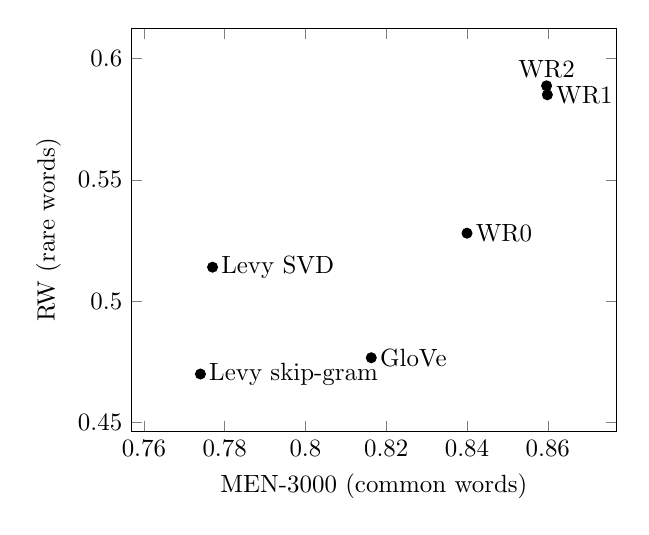
\begin{tikzpicture}[scale=.9]
    \begin{axis}[enlargelimits=0.2, xlabel={MEN-3000 (common words)}, ylabel={RW (rare words)}]
        \addplot[
          scatter,mark=*,only marks,nodes near coords,
          point meta=explicit symbolic,
          visualization depends on={value \thisrow{anchor}\as\myanchor},
          every node near coord/.append style={anchor=\myanchor}
        ]
        table[meta=label] {
            x      y     label             anchor
            .777   .514  {Levy SVD}        west
            .774   .470  {Levy skip-gram}  west
            .8163  .4767 {GloVe}           west
            .8400  .5280 {WR0}             west
            .8599  .5850 {WR1}             west
            .8597  .5887 {WR2}             south
        };
    \end{axis}
\end{tikzpicture}
\caption{
    Systems discussed in this paper, plotted according to their $\rho$
    correlation with MEN-3000 and RW.
}
\label{compare-graph}
\end{figure}


We have labeled some of the rows of Table~\ref{eval-bigtable} as particular systems
that we would like to compare. System {\bf G} represents a configuration of
GloVe that was evaluated by \newcite{pennington2014glove}. We ran the evaluation
using their provided data, and successfully reproduced their results.

{\bf WR1} and {\bf WR2} are two preferred configurations of our system. {\bf WR1}
applies all the techniques described in this paper as it retrofits with
ConceptNet; {\bf WR2} is the same, but retrofits with a combination of PPDB and
ConceptNet. Both systems perform very well across all word-similarity
evaluations, and it is inconclusive which one is better. We will focus on
system {\bf WR1} for further comparison, because it is simpler.

The numerals in the names {\bf WR1} and {\bf WR2} refer to the number of
additional data sources that were added to the original data using our expanded
version of retrofitting. Another interesting result to compare is {\bf WR0},
the best system that we created without retrofitting anything. This system
simply involves transforming the rows and columns of the existing GloVe 840B
matrix, showing that some of the improvements from this paper can be realized
without introducing any additional data.

Table~\ref{eval-multilingual} shows the performance of these systems on
gold standards that have been translated to other languages, in comparison to
the multilingual results published by \newcite{faruqui2015retrofitting}.
These systems perform well in German, French, and Spanish, even though only
German has a data source designed for it in ConceptNet. French and Spanish terms
are only available because of translations in the English Wiktionary, and
indirect translations via Japanese in JMDict.

In contrast, we also briefly tried evaluating on the Arabic and Romanian
translations from \newcite{hassan2009crosslingual}. These languages are not
currently well-represented in ConceptNet, and their preliminary evaluation
results were quite poor.

\subsection{Comparisons to Other Published Results}

\begin{table*}[t]
\centering
\begin{tabular}{lrrrrrr}
\toprule
Label   & RW [dev] & RW [test] & RW [all] & MEN [dev] & MEN [test] & MEN [all]\\
\midrule
\bf G   &    .489  &    .448  &    .477  &    .813  &    .816 &    .814 \\
\bf WR0 &    .536  &    .512  &    .528  &    .841  &    .840 &    .841 \\
\bf WR1 &    .587  &    .581  &    .585  &\bf .858  &\bf .860 &\bf .859 \\
\bf WR2 &\bf .591  &\bf .584  &\bf .589  &    .857  &\bf .860 &    .858 \\
\bottomrule
\end{tabular}

\caption{
    A comparison of evaluation results between the ``dev'' datasets that were
    used in development, and the held-out ``test'' datasets, for the systems
    labeled in Table~\ref{eval-bigtable}.
}
\label{eval-dev-test}
\end{table*}

\begin{table*}[t]
\centering
\begin{tabular}{lrrrrrr}
\toprule
Modification & RW [dev] & MEN [dev] & WS-353 & SCWS &  RG-65 &  MC-30 \\
\midrule
{\bf Unmodified}                     & \bf .587 & \bf .858 & \bf .818 &  .668 &   .852 &   .845 \\
Use first row instead of row-merging & .563 &      .827 &    .787 &  .649 &   .822 &   .794 \\
Unweighted row-merging               & .526 &      .844 &    .751 &  .586 &   .841 &   .836 \\
No self-loops in retrofitting        & .570 &      .855 &    .790 & \bf .676 & \bf .873 & \bf .853 \\
Don't rebalance ConceptNet sources   & .584 &      .854 &    .816 &  .668 &   .846 &   .842 \\
\bottomrule
\end{tabular}
\caption{
    The effects of various modifications to the embeddings of system {\bf WR1}.
    RW and MEN-3000 were evaluated using their development sets here,
    not the held-out test data.
}
\label{eval-variations}
\end{table*}

In Table~\ref{compare-others}, we compare our results on the RW and MEN-3000
datasets to the best published results that we know of.
\newcite{levy2015embeddings} present results including an SVD-based method
that scores $\rho = .514$ on the RW evaluation, as well as an implementation
of skip-grams with negative sampling (SGNS), originally introduced by
\newcite{mikolov2013word2vec}. We also compare to the original results from
GloVe's 42-billion-token dataset.

In relative terms, the performance of our system {\bf WR2} outperforms the best
published RW score (Levy's SVD) by 14.6\%, or 13.6\% if we use our score on only
the test set. Both {\bf WR1} and {\bf WR2} outperform GloVe's result on
MEN-3000 by 5.4\%.

\section{Discussion}

\subsection{Standardizing Term Texts}

When applying ConceptNet's standardization procedure to the labels of GloVe's
840B-token dataset, we found an unexpected benefit from cleaning up that data in
the form of a very large performance increase on the rare words evaluation,
even before retrofitting anything onto it.

When we run our evaluation without modifying the labels on the GloVe 42B-token
embeddings, we reproduce the results published in \cite{pennington2014glove}.
This same evaluation, when run on the 840B-token embeddings, produces
surprisingly poor results, implying that some of these rare words appear in
forms that have low-quality embeddings. When we standardize the GloVe labels and
combine them using the Zipf estimate, however, the result outperforms the
42B-token embeddings.

We conclude from this that it is important to combine the information learned
from multiple forms of a word, including differences in inflection and
capitalization, instead of relying on a single word form to have the correct
vector. However, even if too many word forms were distinguished in the GloVe
learning process, re-combining the word forms after the fact is sufficient to
repair the data.

\subsection{Varying the System}

Some of the procedures we implemented in creating systems {\bf WR1} and
{\bf WR2} require some justification. To show the benefits of certain decisions,
such as adding self-loops or the way we choose to merge rows of GloVe, we have
evaluated what happens to the system in the absence of each decision. These
evaluations appear in Table~\ref{eval-variations}. These evaluations were
part of how we decided on the best configuration of the system, so they were
run on the development sets of RW and MEN-3000, not the held-out test sets.

In Table~\ref{eval-variations}, we can see that the choice of how to merge rows
of GloVe that get the same standardized label makes a large difference.  Recall
that the method we ultimately used was to assign each row a pseudo-frequency
based on Zipf's law, and taking a weighted average based on those frequencies.
The results drop noticeably when we try the other proposed methods, which are
taking only the first (most frequent) row that appears, or taking the
unweighted average of the rows.

In the retrofitting procedure, we made the decision to add ``self-loops'' that
connect each term to itself, hypothesizing that this would help stabilize the
representations of terms that are outside the original vocabulary of GloVe.
Reversing this decision causes a noticeable drop in performance on RW, the
evaluation that is most likely to involve words that were poorly represented or
unrepresented in GloVe. On the other hand, the lack of self-loops seems to {\em
increase} its score on SCWS, and on the smaller evaluations RG-65 and MC-30.

Rebalancing the weights of the data sources within ConceptNet seems to have
been a mild improvement. The ``Don't rebalance'' row of Table~\ref{eval-variations}
confirms what we saw when we introduced rebalancing,
as leaving the weights unbalanced decreases the scores slightly.

In separate experimentation, we found that when we separate ConceptNet into its
component datasets and drop each one in turn, the effects on the evaluation
results are mostly quite small. There is no single dataset that acts as the
``keystone'' without which the system falls apart, but one dataset ---
Wiktionary --- unsurprisingly has a larger effect than the others, because it
is responsible for most of the assertions. Of the 5,631,250 filtered assertions
that come from ConceptNet, 4,244,410 of them are credited to Wiktionary.

Without Wiktionary, the score on RW drops from .587 to .541. However, at the
same time, the MEN-3000 score {\em increases} from .858 to .865. The system
continues to do what it is designed to do without Wiktionary, but there seems to
be a tradeoff in performance on rare words and common words involved.

\subsection{The Limits of Similarity Judgments}

\newcite{bruni2014men} describe a substitute for inter-annotator agreement on
their MEN-3000 dataset:

\begin{quote}
``The Spearman correlation of the two authors is at 0.68, the correlation of their
average ratings with the MEN scores is at 0.84. On the one hand, this high
correlation suggests that MEN contains meaningful semantic ratings. On the
other, it can also be taken as an upper bound on what computational models can
realistically achieve when simulating the human MEN judgments.''
\end{quote}

Our model achieves a MEN score of \scoreMEN{} on the
held-out test data, putting its performance above that upper bound. In many
circumstances, this would be an indication that the model has overfit to the
MEN data. However, we have tried to eliminate the possibility of overfitting.
The MEN data is never used as an input to the system; the same system also
achieves good results on all other data sets; and we did not use or even
look at the held-out data when setting parameters. Strikingly, the evaluation
score on MEN goes {\em up} when the held-out data is evaluated instead.

We postulate instead that similarity evaluations become easier to match
computationally when averaged over the judgments of many people. Notice, for
example, that the two MEN-3000 authors who provided their own ratings
agreed more with the average of the crowd than they did with each other.
If more people's judgments had been averaged in with the authors, perhaps the
correlation would have been even higher. We suspect that, while these results
may be approaching it, the true upper bound of the MEN evaluation is higher than
claimed.

\subsection{Future Work}

% TODO: make these paragraphs flow together?

One aspect of our method that clearly has room for improvement is the fact that
we disregard the labels on relations in ConceptNet, and exclude antonym
relations altogether. There is valuable knowledge there that we might be able
to take into account with a more sophisticated extension of retrofitting, one
that goes beyond simply knowing that particular words should be related, to
handling them differently based on {\em how} they are related.

It was convenient, but not entirely correct, to assume that all of GloVe's data
from the Common Crawl is in English. The Common Crawl is in a wide variety of
languages, just as the Web itself is. In our system, non-English terms are
represented only by links in ConceptNet, but we could have a better starting
point if multilingual terms were represented in the GloVe vectors in the first
place. It could be useful to re-run GloVe in a way that distinguishes languages,
using the metadata on Web pages when available and language-detection heuristics
otherwise.

We believe that the variety of data sources represented in ConceptNet helped to
improve evaluation scores by expanding the domain of the system's knowledge.
There's no reason the improvement needs to stop here. It is quite likely that
there are more sources of ``linked data'' that could be included, or further
standardizations that could be applied to the text to align more data. In
short, these results can probably be surpassed soon. As the second author
observed while running evaluations, ``It seems like every time we do {\em
anything} to the data, the results get better.''

\section{Reproducing These Results}

We aim for these results to be reproducible and reusable by others. The code
that we ran to produce the results in this paper is available in a GitHub
repository at [{\em currently private pending blind review}]. We have tagged
this revision as [{\em TBD}], as we intend to continue to revise and improve the
code afterward. The data files are available at [{\em TBD}], and the README file
in the repository explains how to use {\tt git-annex} to connect the code
with a version-controlled snapshot of the data.

\begin{CJK*}{UTF8}{min}
\bibliography{wordsim_paper}
\end{CJK*}

\end{document}
